\begin{frame}{The world guard destroyed reflected photons}
\begin{columns}[T]
\column{\HalfWidth}
The old rule killed optical tracks by the post-step name \texttt{WorldLV}, without consulting the boundary status.
\begin{block}{Observed at BarPV $\to$ WorldPV}
\BarWorldCount\ encounters;\\
\KilledTirCount\ were TIR: \alert{\TirFraction\%}.
\end{block}
A reflected step can still name WorldPV as its post-step volume. The corrected guard checks the boundary status.
\column{\HalfWidth}
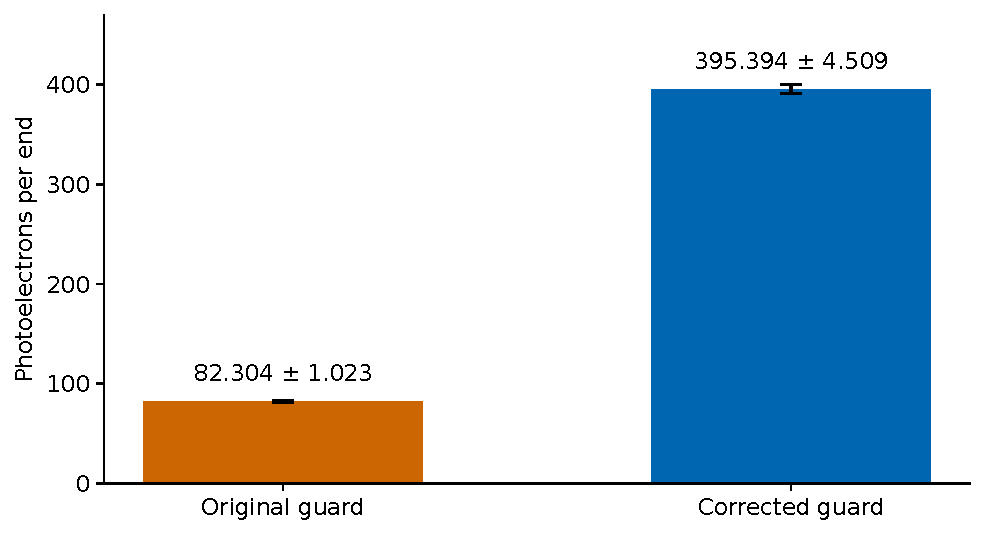
\includegraphics[width=\linewidth]{figs/guard_yields.pdf}
\centering $N=\GuardN$ in \emph{both} arms; error bars are event-level SEM.
\end{columns}
\Source{\GuardSource}
\end{frame}
